\section{UML Diagramme}

\begin{bonus}{UML Diagramme}
    \begin{tabular}{|l|l|l|}
        \hline
        \multirow{2}{*}{Strukturdiagramme} & \multicolumn{2}{c|}{Verhaltensdiagramme}                                 \\\cline{2-3}
                                           &                                          & Interaktionsdiagramme         \\\hline
        Klassendiagramm                    & Use-Case-Diagramm                        & Sequenzdiagramm               \\
        Paketdiagramm                      & Aktivitätsdiagramm                       & Kommunikationsdiagramm        \\
        Objektdiagramm                     & Zustandsautomaten                        & Timingdiagramm                \\
        Kompositionsstrukturdiagramm       &                                          & Interaktionsübersichtdiagramm \\
        Komponentendiagramm                &                                          &                               \\
        Verteilungsdiagramm                &                                          &                               \\\hline
    \end{tabular}
\end{bonus}

\subsection{Use-Case-Diagramm}

\begin{defi}{Use-Case-Diagramm}
    \emph{Use-Case-Diagramme} ermöglichen einen einfachen Einstig in die Projektanalyse.
    Des Weiteren zeigen diese das externe Verhalten eines System aus Sicht der Nutzenden, und wie diese mit dem System interagieren um ein Zeil zu erreichen.

    Des weiteren soll das Use-Case Diagramm antworten auf folgende Fragen liefern:
    \begin{itemize}
        \item \emph{Was} soll mein System für seine Umwelt\footnote{Stakeholder, Nachbarsysteme etc.} leisten?
        \item Welche Interaktionsmöglichkeiten zwischen dem System und den Benutzenden sind für ein bestimmtes Ziel definiert.
        \item Durch hohe Kontextabgrenzung entsteht ein hohes Abstraktionsniveau trotz einer einfachen bzw. schlichten Notation.
    \end{itemize}
\end{defi}

\begin{defi}{Use-Case-Diagramm (Aufbau)}
    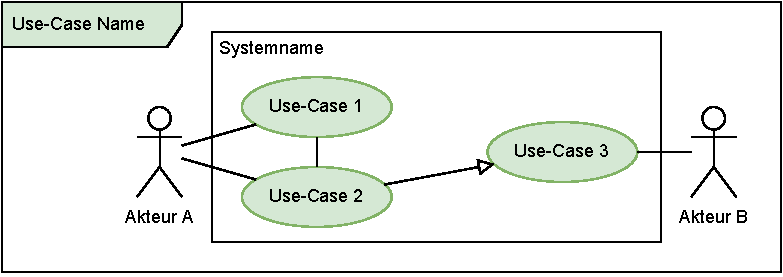
\includegraphics[width=\textwidth]{includes/figures/defi_diagrams_use_case_intro.pdf}

    Anbei findet man eine tabellarische textuelle Beschreibung jedes relevanten Anwendungsfalls:

    \begin{tabularx}{\textwidth}{|>{\bfseries}l|X|}
        \hline
        \multicolumn{2}{|l|}{Use-Case-Nummer, Use-Case-Name}                                                                                                 \\\hline\hline
        Kurzbeschreibung  & ein kurzer erklärender strukturierter Satz zur Übersicht                                                                         \\\hline
        Akteure           & Personen bzw. Rollen oder externe Systeme, die aktiv mit dem System interagieren oder einen Nutzen von dem Anwendungsfall haben.
        Ein Anwendungsfall kann mit mehreren Akteuren verbunden sein.                                                                                        \\\hline
        Kategorie         & muss, soll oder kann der Anwendungsfall realisiert werden                                                                        \\\hline
        Auslösung         & ein Akteur oder eine Funktion, die den Ablauf startet                                                                            \\\hline
        Vorbedingung      & eine Bedingung, die erfüllt sein muss, damit der Ablauf gestartet wird                                                           \\\hline
        Eingabe / Ausgabe & für den Ablauf benötigte Informationen / Ergebnis des Ablaufs                                                                    \\\hline
        Nachbedingung     & Eine Bedingung, die erfüllt sein muss, um den Anwendungsfall zu beenden                                                          \\\hline
        Ablauf            & beschreibt den Standardablauf - keine Sonderfälle                                                                                \\\hline
    \end{tabularx}
\end{defi}

\begin{defi}{Akteur (Use-Case-Diagramm)}
    \begin{wrapfigure}{r}{0.15\textwidth}
        \centering
        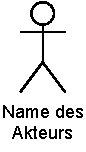
\includegraphics[width=0.1\textwidth]{includes/figures/defi_diagrams_use_case_akteur.pdf}
    \end{wrapfigure}
    %
    Personen oder Rollen werden meist durch Akteure beschreiben.

    In Use-Case Diagrammen stoßen diese Akteure Anwendungsfälle an.

    Alternativ stehen neben dem stilisiertem Symbol weitere Rollen-spezifische Symbole zur Verfügung:

    \begin{center}
        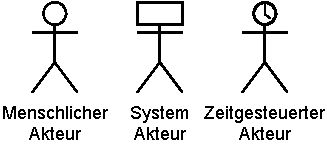
\includegraphics[width=0.4\textwidth]{includes/figures/defi_diagrams_use_case_akteur_types.pdf}
    \end{center}
\end{defi}

\begin{bonus}{Spezifischer Akteur (Use-Case-Diagramm)}
    \begin{wrapfigure}{r}{0.35\textwidth}
        \centering
        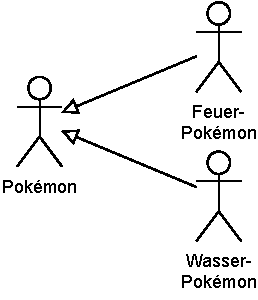
\includegraphics[width=0.3\textwidth]{includes/figures/bonus_diagrams_use_case_akteur_specification.pdf}
    \end{wrapfigure}
    %
    Wenn Akteure durch bestimmte Eigenschaften erweitert werden müssen, jedoch in ihrer Grundform weiterhin benötigt werden, kann man diese spezifische Rollen durch allgemeinen Rollen generalisieren\footnote{Vergleichbar mit Vererbung in objektorientierter Programmierung}.

    Dementsprechend wird hier der Akteur \emph{Pokémon} durch \emph{Feuer-} sowie \emph{Wasser-Pokémon} spezialisiert.

    \vspace{7em}
\end{bonus}

\begin{defi}{Use-Case (Use-Case-Diagramm)}
    \begin{wrapfigure}{r}{0.25\textwidth}
        \centering
        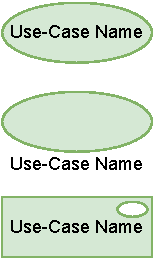
\includegraphics[width=0.2\textwidth]{includes/figures/defi_diagrams_use_case.pdf}
    \end{wrapfigure}
    \emph{Use-Cases} bzw. Anwendungsfälle beschreiben eine Aktivität.
    Dabei besteht der Name aus einem Substantiv und einem Verb.

    z.B. würde \enquote{Pokémon fangen} diese Namenskonvention erfüllen.

    Diese werden meist mit einem Oval oder einer Ellipse dargestellt.
    Dabei steht der Name - je nach vorhandenem Platz - entweder in dem Symbol oder darunter.

    \vspace{2.5cm}
\end{defi}

\begin{defi}{Systeme und Grenzen (Use-Case-Diagramm)}
    Um das Gesamtsystem aus fachlicher Sicht einzuordnen, kann man Anwendungsfalls-Gruppen in einem \emph{System} zusammenfügen.
    Diese Systeme grenzen verschiedene fachliche Teile, Aufgaben und/ oder Verantwortungsbereiche voneinander ab.

    %Dabei dient die Einteilung nicht als technische Analyse!
\end{defi}

\begin{defi}{Kanten bzw. Assoziationen (Use-Case-Diagramm)}
    \emph{Kanten bzw. Assoziation} modellieren Interaktionen zwischen:
    \begin{itemize}
        \item Akteur und Akteur
        \item Akteur und Use-Case
        \item Use-Case und Use-Case
    \end{itemize}
    und beantworten die Frage, wer mit wem in welcher Beziehung steht.

    Dabei erfolgt die Darstellung über Kanten und Linien, welche ggf. über Zusätzliche Annotationen angereichert werden.
\end{defi}

\begin{defi}{Zusammenfassung Assoziationstypen (Use-Case-Diagramm)}
    \begin{itemize}
        \item Binäre Assoziation (ungerichtet)

              Richtung nicht eindeutig, i.d.R. ausgehend von einem der beteiligten Akteuren

              \vspace{1em}
              \begin{center}
                  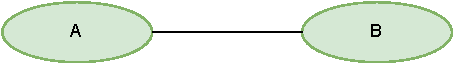
\includegraphics[width=0.5\textwidth]{includes/figures/defi_diagrams_use_case_assoziation.pdf}
              \end{center}

        \item Import/ Include Beziehung

              \emph{A} \emph{umfasst} das Verhalten von \emph{B} vollständig.
              D.h. B ist eine Teilfunktion von A.
              A beinhaltet aber noch weitere Teile.
              Dies ist eine klassische Anwendung um Redundanzen zu vermeiden:
              Mehrere Use-Cases führen denselben Teil aus, dann wird er ausgelagert und gemeinsam genutzt.

              \vspace{1em}
              \begin{center}
                  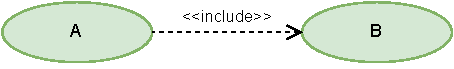
\includegraphics[width=0.5\textwidth]{includes/figures/defi_diagrams_use_case_include.pdf}
              \end{center}

        \item Erweiterungsbeziehung

              \emph{A} \emph{erweitert} \emph{B} unter einer speziellen Voraussetzung

              \vspace{1em}
              \begin{center}
                  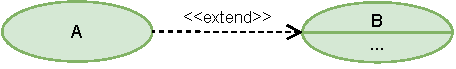
\includegraphics[width=0.5\textwidth]{includes/figures/defi_diagrams_use_case_extend.pdf}
              \end{center}

        \item Generalisierungsbeziehung

              \emph{A} ist ein \emph{B}.
              Interessant bei abstrakten Akteuren und / oder Teilsystemen.

              \vspace{1em}
              \begin{center}
                  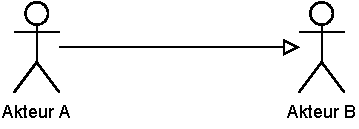
\includegraphics[width=0.4\textwidth]{includes/figures/defi_diagrams_use_case_generalisierung.pdf}
              \end{center}
    \end{itemize}

    Obacht: Bei der Angabe mehrerer Assoziationen ist die Reihenfolge nicht festgelegt.
\end{defi}

\begin{example}{Use-Case-Diagramm}
    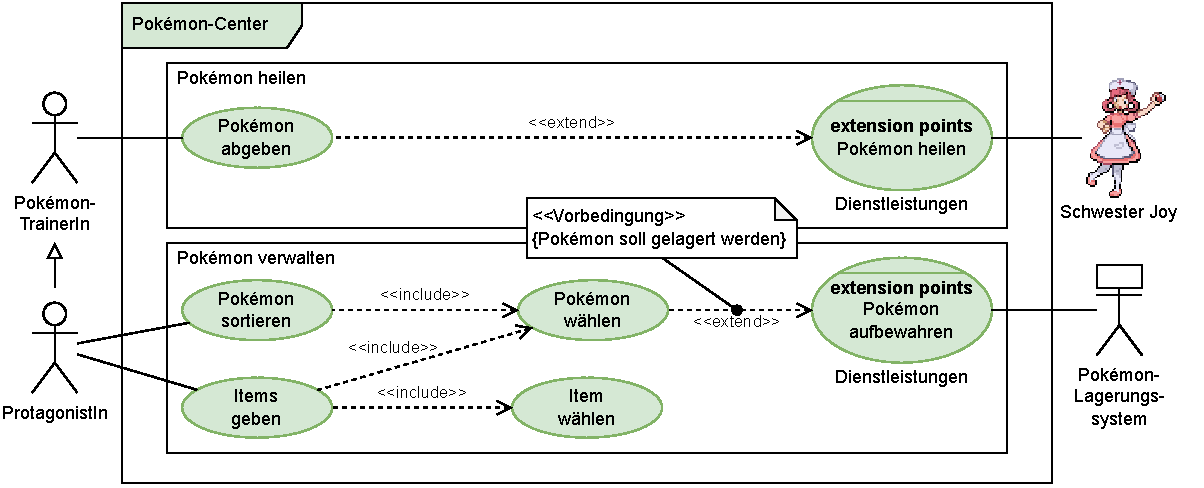
\includegraphics[width=\textwidth]{includes/figures/example_diagrams_use_case.pdf}
\end{example}

\begin{example}{Use-Case-Diagramm (Textuelle Beschreibung)}
    \begin{tabularx}{\textwidth}{|>{\bfseries}l|X|}
        \hline
        \multicolumn{2}{|l|}{UC2: Pokémon sortieren}                                                                           \\\hline\hline
        Kurzbeschreibung  & Verwaltet das aktuelle Team und tauscht - falls nötig - Pokémon aus dem Pokémon-Lagerungsystem ein \\\hline
        Akteure           & ProtagonistIn                                                                                      \\\hline
        Kategorie         & kann                                                                                               \\\hline
        Auslösung         & Entscheidung das Team zu modifizieren                                                              \\\hline
        Vorbedingung      & mind. zwei Pokémon im Team bzw. in der Box vorhanden                                               \\\hline
        Eingabe / Ausgabe & E: Altes Team, Modifikation, A: Neues Team                                                         \\\hline
        Nachbedingung     & Pokémon wurden gewählt und getauscht                                                               \\\hline
        Ablauf            & \begin{enumerate}
                                \item ProtagonistIn betritt das Pokémon-Center
                                \item ProtagonistIn meldet sich am Pokémon-Lagerungsystem an
                                \item Solange ProtagonistIn nicht fertig
                                      \begin{enumerate}
                      \item Wähle auszutauschendes Pokémon
                      \item Wähle einzutauschendes Pokémon
                  \end{enumerate}
                            \end{enumerate}                                        \\\hline
    \end{tabularx}
\end{example}

\subsection{Aktivitätsdiagramm}

\begin{defi}{Aktivitätsdiagramm}
    Primär beantworten \emph{Aktivitätsdiagramme} die Frage, \emph{wie} etwas realisiert werden soll.
    Sie stellen konkrete komplexe Abläufe dar, indem sie diese wie folgt zerlegen:
    \begin{itemize}
        \item Nebenläufe
        \item alternative Entscheidungswege
        \item Einzelschritte von Aufgaben
    \end{itemize}

    Aktivitätsdiagramme können für folgende Objekte genutzt werden:
    \begin{itemize}
        \item einen Use-Case
        \item eine Operation
        \item ein Geschäftsmodell
    \end{itemize}
\end{defi}

\begin{defi}{Aktivitätsdiagramm (Aufbau)}
    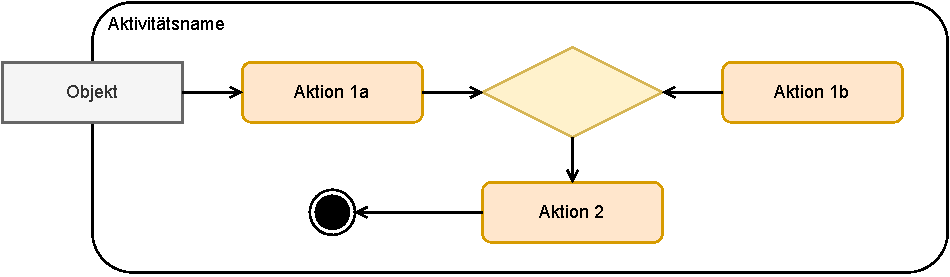
\includegraphics[width=\textwidth]{includes/figures/defi_diagrams_activity_intro.pdf}
\end{defi}

\begin{defi}{Aktivität (Aktivitätsdiagramm)}
    Gesamtheit aller Abläufe eines Kontexts
\end{defi}

\begin{defi}{Aktion (Aktivitätsdiagramm)}
    \begin{wrapfigure}{r}{0.25\textwidth}
        \centering
        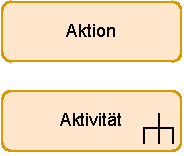
\includegraphics[width=0.2\textwidth]{includes/figures/defi_diagrams_activity_aktion.pdf}
    \end{wrapfigure}
    Eine \emph{Aktion} ist ein Einzelschritt, den ein Ablauf unter Zeitaufwand durchschreitet.

    Aktionen können in einem Aktivitätsdiagramm eine weitere Aktivität aufrufen.
    Dies kennzeichnet man durch eine \enquote{stilisierte Harke}.

    In diesen Unteraktivitäten können Eingangs- sowie Ausgangs-Parameter durch Objektknoten festgelegt werden.
\end{defi}

\begin{defi}{Objektknoten (Aktivitätsdiagramm)}
    \begin{wrapfigure}{r}{0.25\textwidth}
        \centering
        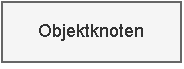
\includegraphics[width=0.2\textwidth]{includes/figures/defi_diagrams_activity_objektknoten.pdf}
    \end{wrapfigure}
    Beteiligte Daten / Schnittstellen einer Aktion

    \vspace{1cm}
\end{defi}

\begin{defi}{Verbindende Kanten}
    Verlaufsweg mögl. Programmflüsse.
    Dient der Übertragung erstellter Tokens sowie Objekten.
\end{defi}

\begin{defi}{Kontrollelemente zur Ablaufsteuerung (Aktivitätsdiagramm)}
    \begin{wrapfigure}{r}{0.25\textwidth}
        \centering
        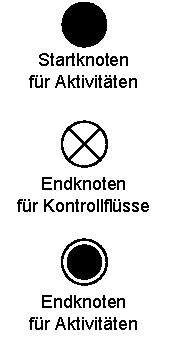
\includegraphics[width=0.175\textwidth]{includes/figures/defi_diagrams_activity_start_end.pdf}
    \end{wrapfigure}
    \textbf{Startknoten:}
    \begin{itemize}
        \item Markiert den Startpunkt eines Ablaufs beim Aktivieren einer Aktivität
        \item Eine Aktivität kann beliebig viele Startknoten haben (Nebenläufige Ausführung an allen Startknoten)
        \item Eine Aktivität muss keinen Startknoten besitzen (Eingabeparameter dienen als Startpunkt)
        \item Jeder Startknoten erstellt ein Token, welches der anliegenden Kante mitgegeben wird.
    \end{itemize}

    \textbf{Endknoten für Kontrollflüsse:}
    \begin{itemize}
        \item Beendet nur einen einzelnen Ablauf, indem das aktuell anliegende Token gelöscht wird.
        \item Nebenläufig ausgeführte Aktionen werden nicht beendet.
        \item Beendigung der gesamten Aktivität daher nur bei nicht parallelisierten Abläufen
    \end{itemize}

    \textbf{Endknoten für Aktivitäten:}
    \begin{itemize}
        \item Beendet sofort die gesamte Aktivität, indem alle Tokens gelöscht werden.
        \item Parallel ausgeführte Aktionen werden ebenfalls beendet
    \end{itemize}
\end{defi}

\begin{defi}{Kontrollelemente zur Ablaufsteuerung für Bedingungen (Aktivitätsdiagramm)}
    \begin{wrapfigure}{r}{0.25\textwidth}
        \centering
        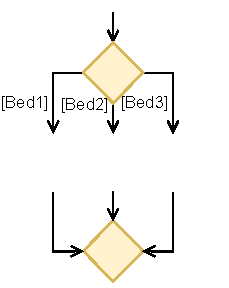
\includegraphics[width=0.2\textwidth]{includes/figures/defi_diagrams_activity_or.pdf}
    \end{wrapfigure}
    \textbf{Verzweigungsknoten:}
    \begin{itemize}
        \item Spaltet eine Kante in mehrere Alternativen auf.
              Dabei kann der Verzweigungsknoten \emph{maximal einen} Token weitergeben.
        \item Programmfluss wird von Bedingungen abhängig gemacht.
        \item Bei mehreren ausgehenden Kanten müssen alle Bedingungen disjunkt sein.
    \end{itemize}

    \textbf{Verbindungsknoten}
    \begin{itemize}
        \item Führt mehrere unabhängige Kanten in einem gemeinsamen Programmfluss zusammen.
              Dabei ist es egal, wie viele Token aus welchen Kanten ankommen - jedes Token wird von dem Verbindungsknoten direkt weitergeleitet.
    \end{itemize}
\end{defi}

\begin{defi}{Kontrollelemente zur Ablaufsteuerung zur Parallelisierung (Aktivitätsdiagramm)}
    \begin{wrapfigure}{r}{0.25\textwidth}
        \centering
        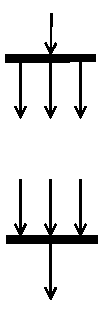
\includegraphics[width=0.1\textwidth]{includes/figures/defi_diagrams_activity_and.pdf}
    \end{wrapfigure}
    \textbf{Parallelisierungsknoten}
    \begin{itemize}
        \item Teilt den Ablauf einer eingehenden Kante in mehrere parallele Abläufe auf.
              Dabei muss der Parallelisierungsknoten \emph{exakt so viele} Tokens weitergeben, wie ausgehenden Kanten vorhanden sind.
        \item Ermöglicht Nebenläufigkeit von Aktionen.
        \item Kontroll- bzw. Objektfluss muss am Ende wieder zusammengefasst oder getrennt werden.
    \end{itemize}

    \textbf{Synchronisationsknoten:}
    \begin{itemize}
        \item Vereint parallele Abläufe.
              Dabei muss aus jeder eingehenden Kante \emph{mindestens ein} Token empfangen werden.
              Diese werden im Anschluss gebündelt weitergeleitet.
    \end{itemize}
\end{defi}

\begin{defi}{Signale und Ereignisse zur Parallelisierung (Aktivitätsdiagramm)}
    \begin{wrapfigure}{r}{0.25\textwidth}
        \centering
        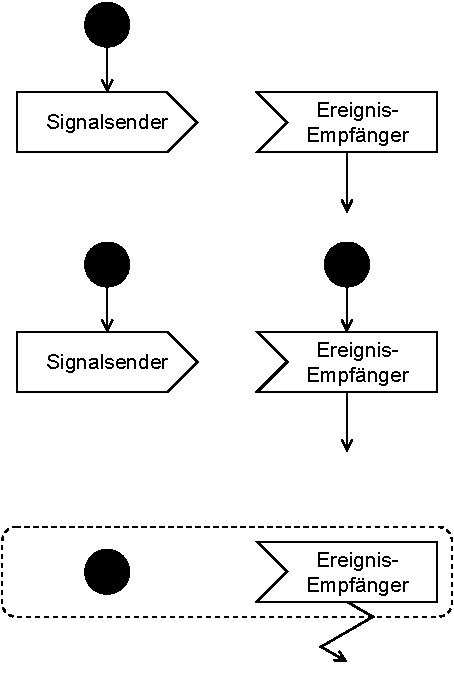
\includegraphics[width=0.25\textwidth]{includes/figures/defi_diagrams_activity_signal.pdf}
    \end{wrapfigure}
    \textbf{Signal Sender:}
    \begin{itemize}
        \item Löst die Sonderaktion \emph{SendSiganlAction} aus, sobald ein Token das Objekt erreicht.
    \end{itemize}

    \textbf{Ereignisempfänger:}
    \begin{itemize}
        \item Löst die Sonderaktion \emph{AcceptEventAction} aus, sobald ein Signal gesendet wurde.
        \item Diese Objekte erscheinen in drei Variationen:
              \begin{itemize}
                  \item Ereignisempfänger \emph{ohne einlaufende Kante}

                        Dieser reagiert unmittelbar nach Erhalt des Sendesignals wie eine normale Aktion.
                  \item Ereignisempfänger \emph{mit einlaufender Kante}

                        Dieser reagiert erst, wenn sowohl ein Sendesignal empfangen wurde, als auch ein Token durch die anliegende Kante erhalten wurde.
                  \item Ereignisempfänger \emph{mit Unterbrechungskante}

                        Dieser reagiert unmittelbar nach Erhalt des Sendesignals.
                        Zusätzlich wird der Gruppierungsbereich\footnote{Anliegende gestrichelte Linie} unterbrochen, und der Programmfluss wird am Ende der anliegenden Unterbrechungskante fortgesetzt.
              \end{itemize}
    \end{itemize}
\end{defi}

\subsection{Klassendiagramm}

\begin{defi}{Klassendiagramm}
    Klassendiagramme existieren in zwei verschiedenen Formen:

    \begin{itemize}
        \item Klassendiagramm für Analysemodell
              \begin{itemize}
                  \item Klassen
                  \item Attribute
                  \item Assoziationen / Vererbung / Multiplizitäten
                  \item Kompositionen / Aggregationen
              \end{itemize}
        \item Klassendiagramm für Entwurfsmodell (erweitert das Analysemodell)
              \begin{itemize}
                  \item Operationen bzw. Methoden / Funktionen
                  \item Klassen- und Objekteigenschaften
                  \item Abgeleitete Eigenschaften Sichtbarkeiten
                  \item Navigationsrichtungen
                  \item Eigenschaften von Attributen und Assoziationsenden
                  \item Qualifizierte Assoziationen
                  \item Klassenarten
                  \item Abhängigkeiten
              \end{itemize}
    \end{itemize}
\end{defi}

% \begin{defi}{Klassendiagramm (Aufbau)}
%     \begin{center}
%         \includegraphics[width=0.35\textwidth]{includes/figures/03_class_diagram.pdf}
%     \end{center}
% \end{defi}

\begin{defi}{Klasse (Klassendiagramm)}
    \begin{wrapfigure}{r}{0.25\textwidth}
        \centering
        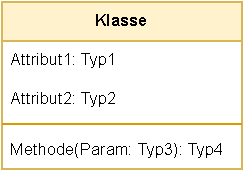
\includegraphics[width=0.25\textwidth]{includes/figures/defi_diagrams_class_intro.pdf}
    \end{wrapfigure}
    UML \emph{Klassen} entsprechen den programmatischen Klassen aus bekannten objektorientierten Sprachen.

    Das Symbol besteht aus einem Header mit dem großgeschriebenen fettgedruckten horizontal mittig zentrierten Klassennamen und zwei \enquote{Containern}.
    Diese werden mit potentiellen Attributen (oben) und Operationen bzw. Methoden (unten) der Klasse gefüllt.

    Hier werden einige weitere Symbole bzw. Schlüsselworte benötigt\footnote{default ist \texttt{\textasciitilde \{unordered, unique\}}}:
    \begin{itemize}
        \item Sichtbarkeit:
              \subitem + : \texttt{public}
              \subitem - : \texttt{private}
              \subitem \# : \texttt{protected}
              \subitem \textasciitilde\ : \texttt{package}
              \subitem / : Abgeleitetes Attribut
        \item \texttt{\{id\}} : Attribut entspricht einem Primärschlüssel
        \item \texttt{\{readOnly\}}
        \item \texttt{\{frozen\}} bzw. \texttt{\{immutable\}}
        \item \texttt{\{abstract\}}\footnote{alternativ kann man das jeweilige Objekt in kursiv schreiben}
        \item \texttt{static} : Das jeweilige Objekt muss unterstrichen sein
        \item \texttt{generic} bzw Parametrisiert : Die Klasse wird mit einem kleinen Kasten gekennzeichnet, indem alle generischen Typen zu finden sind.
        \item Kollektionen
              \subitem \texttt{\{ordered\}} oder \texttt{\{unordered\}}
              \subitem \texttt{\{unique\}} oder \texttt{\{nonunique\}}
        \item \texttt{<<interface>>}
        \item \texttt{<<utility>>} : Hilfsklassen (diese werden via \texttt{<<use>> genutzt})
    \end{itemize}
\end{defi}

\begin{defi}{Attribut (Klassendiagramm)}
    Jedes Attribut benötigt eine Typangabe\footnote{Man achte auf die exakte Schreibweise; (Primitive-) Datentypen werden groß- und aus-geschrieben}.

    Der Typ wird nach dem kleingeschriebenen Attributnamen mit einem \texttt{:} angegeben.

    Attribute, welche als Fremdschlüssel für andere Klassen dienen, können ebenfalls aufgeführt werden.
    Alternativ schreibt man die Bezeichnung an die Assoziation.\footnote{Siehe Navigierbarkeit, Erreichbarkeit}

    Multiplizitäten für Kollektionen:

    \begin{tabular}{>{\ttfamily}l>{\ttfamily}lll}
        \multicolumn{1}{l}{Symbol} & \multicolumn{1}{l}{alternativ} & Typ          & {Multiplizität}                       \\
        $[$n..m$]$                 &                                &              & zwischen mindestens n und höchstens m \\
        $[$0..1$]$                 & $[$1$]$                        & optional     & höchstens ein Wert                    \\
        $[$0..*$]$                 & $[$*$]$                        & optional     & beliebig viele Werte                  \\
        $[$1..*$]$                 &                                & erforderlich & beliebig viele Werte
    \end{tabular}
\end{defi}

\begin{defi}{Operation (Klassendiagramm)}
    Unter Operationen fallen alle Klassen-abhängigen Methoden und Funktionen.

    Parametrisierte Konstruktoren müssen dort wie gewöhnliche Operationen aufgeführt werden.

    Eine Operation beinhaltet einen Namen, eine Parameterliste und einen Rückgabetyp.
    Diese folgend folgender Syntax:

    \texttt{<Name> ( <Parameterliste> ) [: <Rückgabetyp>]}

    Die Parameterliste ist eine durch Kommata getrennte Aufzählung von Parametern.
    Parameter werden wie folgt dargestellt:

    \texttt{[Richtung] <Name> : <Typ> [Multiplizität][Standardwert]}

    Unter Richtungen fallen:
    \begin{itemize}
        \item \texttt{in} : Call-by-Value
        \item \texttt{inout} : Call-by-Reference
        \item \texttt{out} : initialisiert den Out-Parameter beim Aufrufen der Operation und stellt diesen in dem Scope, indem die Operation aufgerufen wurde, zur Verfügung.
    \end{itemize}
\end{defi}

\begin{defi}{Navigierbarkeit}
    Eine Assoziation ist dann \emph{navigierbar}, wenn Objekte der adjazenten Klasse erreichbar sind.

    \begin{wrapfigure}{r}{0.25\textwidth}
        \centering
        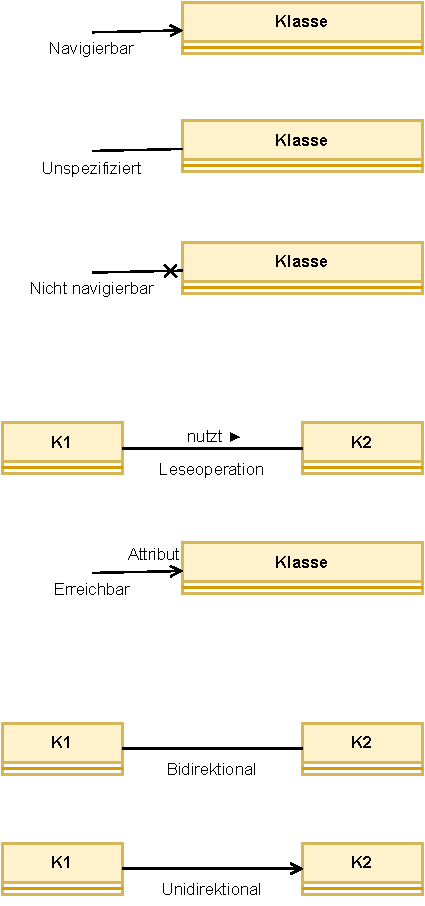
\includegraphics[width=0.25\textwidth]{includes/figures/defi_diagrams_class_assoziation.pdf}
    \end{wrapfigure}
    \textbf{Navigierbarkeit}:

    Dabei hat jede Assoziation eine von drei möglichen Navigationszuständen
    \begin{itemize}
        \item Navigierbar
        \item Unspezifiziert
        \item Nicht navigierbar
    \end{itemize}

    \textbf{Erreichbarkeit}:

    Sollte die Klasse erreichbar sein, muss man eine Leseoperation zur Verfügung stellen.
    Des Weiteren muss man sich überlegen. wie man das Objekt erreichen kann:
    \begin{itemize}
        \item Als Attribut in einer Klasse (siehe rechts)
        \item In Datencontainern wie \texttt{Hashtables}
        \item \ldots
    \end{itemize}

    \textbf{Erreichbarkeitsrichtung}:

    Man unterscheidet Assoziationen wie folgt:
    \begin{itemize}
        \item Unidirektional : Ausschließlich eine Klasse ist erreichbar
        \item Bidirektional : Beide Klassen sind untereinander erreichbar
    \end{itemize}
\end{defi}

\begin{defi}{Generalisierung}
    \begin{wrapfigure}{r}{0.25\textwidth}
        \centering
        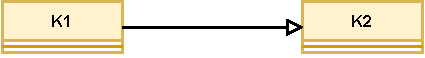
\includegraphics[width=0.25\textwidth]{includes/figures/defi_diagrams_class_vererbung.pdf}
    \end{wrapfigure}
    Eine Generalisierung in der UML ist eine gerichtete Beziehung zwischen einer speziellen und einer genereller Klasse.
    Instanzen der speziellen Klasse sind damit auch Instanzen der generellen Klasse.

    Die Klasse \emph{K1} \emph{erbt} z.B. von der Klasse \emph{K2}.
\end{defi}

\begin{defi}{Aggregation und Komposition}
    \begin{wrapfigure}{r}{0.25\textwidth}
        \centering
        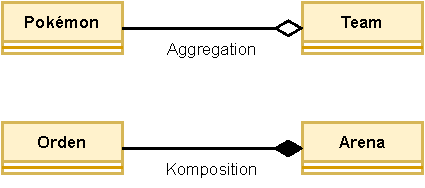
\includegraphics[width=0.25\textwidth]{includes/figures/defi_diagrams_class_aggregation_composition.pdf}
    \end{wrapfigure}
    Zwei Spezialfälle der Assoziation bilden eine Teil/Ganzes-Beziehung.

    \begin{itemize}
        \item \textbf{Aggregation}:

              Ein Objekt (Aggregat) besteht aus mehreren Einzelobjekten.
              Die Lebensdauer der Einzelobjekte kann länger sein als die des Aggregats.
        \item \textbf{Komposition} oder Aggregationskomposition:

              Das Teilobjekt ist von der Existenz des Ganzen abhängig.
              Es kann nicht ohne existieren.
    \end{itemize}
\end{defi}

\begin{defi}{Pakete}
    \begin{wrapfigure}{r}{0.25\textwidth}
        \centering
        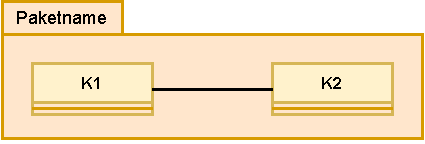
\includegraphics[width=0.25\textwidth]{includes/figures/defi_diagrams_class_package.pdf}
    \end{wrapfigure}
    In der UML dienen \emph{Pakete} zur hierarchisch geschachtelten Strukturierung großer Modelle.
    Jedes Modellelement gehört zu höchstens einem Paket, kann jedoch in mehreren Modellen vorkommen.

    So kann man eine angemessen große Menge modular zerlegter Objekte zu einer logisch geschlossenen Einheit zusammenfassen, welche in größeren Diagrammen genutzt wird.

    Pakete verfolgen das Prinzip der \emph{losen Kopplung} und \emph{hohen Kohäsion}.
\end{defi}

\begin{defi}{Kohäsion}
    \emph{Kohäsion} beschreibt die Kräfte, die ein Modul im Inneren zusammenhalten.

    Eine gewollte starke Kohäsion bedeutet, dass die Teile des Moduls bzw. Pakets eng Zusammenhängen.
    Also werden logische Zusammenhänge ebenfalls strukturell verbunden.
\end{defi}

\begin{defi}{Kopplung}
    \emph{Kopplung} beschreibt die Bindungen, die verschiedene Pakete zusammenhalten.

    Eine gewollte lose (Daten-) Kopplung bewirkt, dass die Module nicht wissen, welche Daten in anderen Modulen gespeichert bzw. berechnet werden.
    Dies wird \emph{Information Hiding} genannt.

    Eine strikte Trennung von Paketen nach dem Prinzip der hohen Kohäsion bewirkt ebenfalls eine lose Kopplung.
    Analog bewirkt lose Kohäsion eine starke Bindung.
\end{defi}

\begin{example}{Kohäsion und Kopplung}
    \begin{wrapfigure}{r}{0.25\textwidth}
        \centering
        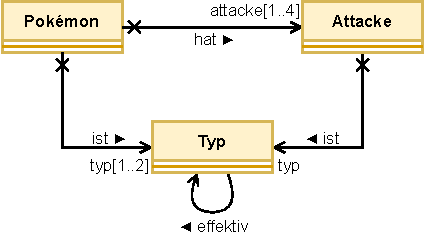
\includegraphics[width=0.25\textwidth]{includes/figures/example_diagrams_class_kohaesion.pdf}
    \end{wrapfigure}
    Beispiel für gewollte starke (funktionale) Kohäsion:
    \begin{itemize}
        \item Die Klassen Pokémon, Typ, Attacke
              \begin{itemize}
                  \item Jedes Pokémon hat mindestens einen Typen.
                  \item Jedes Pokémon hat zusätzlich bis zu vier Attacken.
                  \item Jede Attacke hat ebenfalls einen Typen.
                  \item Jeder Typ ist effektiv gegen andere Typen.
              \end{itemize}

              Wenn man nun eine Klasse aus dem Paket entnimmt und zu einem eigenen Paket macht, erstellt man automatisch 2 Verbindungen zwischen dem aktuellen und dem neuen Paket.
              Da dies eine surjektive Assoziation wäre\footnote{Jedes Element der Zielmenge wird getroffen}, ist hier ein Aufteilen nicht sinnvoll.
    \end{itemize}

    Beispiel für schwache (zufällige) Kohäsion:
    \begin{itemize}
        \item \texttt{getter-}, \texttt{setter-} sowie \texttt{print-} Methoden speichern die Daten des jeweiligen Objekts nicht.
              Dementsprechend kann man diese Methoden im Modell von dem Objekt trennen.
        \item Die Assoziation zwischen Arena bzw. Orden mit der / dem ProtagonistIn.
              \begin{itemize}
                  \item Jede/r ProtagonistIn kann beliebig viele Orden in Arenen freischalten.

                        Hier ist eine Abtrennung eines Arena/Orden-Pakets möglich.
                  \item zwischen Arena und Orden liegt ein hohes Maß an Kohäsion vor.

                        Hier ist eine weitere Trennung nicht sinnvoll.
              \end{itemize}
    \end{itemize}
\end{example}

